\documentclass{article}
\usepackage{amsmath}
\usepackage{natbib}
\usepackage[textwidth=5.8in, textheight=8in]{geometry}
\usepackage{lipsum}
\usepackage[mathscr]{eucal}
\usepackage{graphicx}

\newcommand{\T}{\frac{\theta}{2}}
\newcommand{\E}{\mathrm{E}}
\newcommand{\Var}{\mathrm{Var}}
\newcommand{\Cov}{\mathrm{Cov}}
\newcommand{\Pro}{\mathrm{P}}
\newcommand{\Kurt}{\mathrm{Kurt}}

\begin{document}

\title{Quantitative trait distributions and the coalescent process}
\maketitle

\section{Introduction}
Evolutionary quantitative genetics almost always models phenotypes as normally
distributed. Indeed, it has been suggested that this is the defining
characteristic of the field \citep{Rice2004}. This assumption is of course
well-founded based on Fisher's original demonstration that the observed
continuous distribution of phenotypes and correlations between relatives could
be explained by the action of a large number of Mendelian factors
\citep{Fisher1918}. In this framework the phenotypic distribution at all levels
between individuals, families, populations, and species is completely described
by of a set of means, variances, covariances \citep{Falconer1996}.

Analyses based on infinitesimal-normal models have been powerful tools in many
areas of evolutionary genetics. \citet{Lande1983} used this approach to measure
the action of natural selection on correlated traits over a single generation.
Over much greater time scales, \citet{Freckleton2002} and others used Brownian
motion to detect and correct for phylogenetic dependence in studies of
phenotypic evolution. Classic models of phenotypic evolution have also
incorporated genetic drift by including factors like population size and
subdivision \citep{Chakraborty1982,Lynch1986,Lande1992}. These models have
examined the dynamics of phenotypic evolution forwards in time as a balance
between mutation that creates variance, migration that spreads it among
subpopulations, and fixation that removes it. The focus has been to find
equilibrium genetic variances and the rate at which these are approached.

Of course, there is nothing really remarkable about modeling phenotypes
according to a normal distribution. The point is that trait evolution can be
well studied without worrying about the complex evolutionary dynamics of
particular alleles or the genetic architecture; e.g. the number of loci or
distribution of mutational effects. However, heritable phenotypic variation is
ultimately due to discrete mutations at discrete loci, and how this variation is
distributed depends on the genealogies at these loci. When the number of loci
affecting a trait is large the central limit theorem ensures that most of these
details can be ignored, but a full model would have to include them.

%% Among its many successes, it has been used to find traits under
%% selection in natural populations \citep{Price1984}, determine which dimensions
%% in phenotype space are favored by females during sexual selection
%% \citep{Blows2004}, and test for phylogenetic signal in phenotypic evolution
%% \citep{Freckleton2002}. Such studies and other provide great biological insights
%% without worrying about potentially complex evolutionary dynamics at multiple
%% loci because the entire system can be described in terms of the first and second
%% order moments.

The principle modeling framework for variation in genealogies is the coalescent
process and its varied extensions \citep{Wakeley2008}, but few studies have
connected this with quantitative genetics. The most well-known of these is
\citet{Whitlock1999}, who used a coalescent argument to show that $Q_{ST}$ and
$F_{ST}$ have the same expected value under general models of population
subdivision. \citet{Griswold2007} used coalescent simulations to investigate the
effects of shared ancestry and linkage disequilibrium on the matrix of genetic
variances and covariances between traits ($\mbox{\textbf{G}}$). They found that
the eigenvalues of the expected $\mbox{\textbf{G}}$ and the expected eigenvalues
can be different. Although not explicitly connected to the coalescent,
\citet{Ovaskainen2011} used the formalism of coancestry coefficients to model
the full distribution of correlated traits in related subpopulations. Their main
result was that the covariance in additive genetic values, conditional on the
G-matrix in the ancestral population, depends only on the pairwise coancestry
coefficients.

Most recently, \citet{Schraiber2015} developed a very general model of
quantitative trait evolution based on the coalescent that allows for an
arbitrary distribution of mutational effects and number of loci affecting the
trait. They derived the characteristic function for the distribution of
phenotypic values in a sample and showed how such values can deviate strongly
from normality when the number of loci is small or the mutational distribution
has fat tails.

The results of \citet{Schraiber2015} were derived for a panmictic, constant-size
population. Natural populations are often far from equilibrium and show
considerable spatial structure. In fact, the analysis of quantitative traits in
structured populations is of particular interest when searching for evidence of
local adaptation of the lack thereof. To this end the $Q_{ST}$ paradigm was
developed \citep{Whitlock2008,Spitze1993}. $Q_{ST}$, defined as the ratio of the
variance between subpopulations to the total variance in a quantitative trait,
is compared to $F_{ST}$ which measures the same property for genetic variation.
If $Q_{ST}$ exceeds the $F_{ST}$ for neutral genetic variation then it is
concluded that natural selection has acted to diversify the phenotypes. Modern
extensions of this idea have been developed by \citet{Ovaskainen2011} for
genetic values measured in breeding experiments, and by \citet{Berg2014} for
genetic values measured in GWAS. Understanding the neutral distribution of trait
values at the sample and population level is necessary to interpret the results
of the goodness-of-fit tests used in the $Q_{ST}$ paradigm. 

Here, I generalize the work of \citet{Schraiber2015} to an arbitrary
distribution of coalescent times for which their main result, the characteristic
function of the sampling distribution of phenotypic values, is a special case. I
then show how the normal, infinitesimal model arises by taking appropriate
limits. I then calculate the third and fourth moments of the phenotype
distribution to illustrate how departures from normality depend on both the
genetic architecture and genealogical distributions. Finally, I discuss the
consequences of these results for $Q_{ST}$ tests, the response to selection, and
the inference of genetic architecture.
\section{Notation}
It is useful to first describe the various quantities of interest and the
notation used to describe them. The principle quantities are the quantitative
trait values which we will hereafter refer to these as trait values. The random
vector of trait values in the sampled individuals is $\mathbf{Y}$, and an
element $Y_a$ of $\mathbf{Y}$ is the trait value of individual $a$. The trait
values will be modeled as the change relative to the value in the most recent
common ancestor of the sample. Since we do not know what ancestral value was,
$\mathbf{Y}$ cannot be directly observed. Rather, as deviations from an
ancestral value they determine other summaries one might calculate from measured
phenotypes in a sample.

The random vector of branch lengths describing the genealogy at a locus is
$\mathbf{T}$, and an element $T_{a,b}$ of $\mathbf{T}$ is the branch length
subtending individuals $a$ and $b$. $\omega$ will be used to denote a particular
set of individuals and hence a branch on the genealogy such that $T_\omega$ is
then length of branch $\omega$. $\Omega$ is the set of all possible branches.
For instance, if there are three sampled individuals, $a$, $b$, and $c$, then
$\mathbf{Y}=\{Y_a,Y_b,Y_c\}$,
$\mathbf{T}=\{T_a,T_b,T_c,T_{a,b},T_{a,c},T_{b,c}\}$, and
$\Omega=\{(a),(b),(c),(a,b),(a,c),(b,c)\}$. Realizations of the random trait
values and branch lengths are denoted using the same notation with lowercase
letters.

Another useful piece of notation is for sums of branch lengths. Let $\tau_{a+b}$
be the (random) sum of all branches containing both $a$ and $b$. Conversely,
$\tau_{a/b}$ will be the random sum of all branches containing $a$ and not $b$.
Extensions of this for more than two individuals are also used. The same
notation is used when referring to sets of branch indices. So $\Omega_{a+b}$ and
$\Omega_{a/b}$ would be the sets of branches summed to give $\tau_{a+b}$ and
$\tau_{a/b}$.

Other important quantities define the genetic architecture of the trait. These
are $L$, the number of loci at which mutations affect the trait, and $\T$, the
mutation rate. The moment generating function for the distribution of mutational
effects is written as $\psi()$ and moment $i$ of this distribution is $m_i$.
Moment generating functions for the distribution of branch lengths and
distribution of trait values are $\varphi_{\mathbf{T}}$ and
$\varphi_{\mathbf{Y}}$. The model used is haploid, but we do not expect this to
qualitatively change any conclusions.
\section{The moment generating function for the distribution of trait values}
We now consider the moment generating function (mgf) of the distribution of
trait values, remembering that these are measured relative to the most recent
common ancestor of the sample. Our approach closely follows that of
\citet{Schraiber2015} but expands to arbitrary demographies and population
structure. The distribution of trait values is considered over evolutionary
realizations, that is, over the over the combined random processes of drift and
mutation. The distribution of trait values in a population sample is complex in
its general form. It has a point mass at zero corresponding the possibility that
no mutations affecting the trait occur in the history of the sample.
Correlations between individuals arise because of shared history in the
genealogies at individual loci with discrete topologies as well was where on
these genealogies mutations, whose effects may come from a discrete or
continuous distribution, occur. An analytical expression for the distribution of
trait values does not exist except in very special circumstances. This is the
problem that Fisher's infinitesimal model solves.

However, it is sometimes possible to find the mgf of this distribution or at
least learn something from its form. The mgf for the trait values controlled by
a single nonrecombining locus is defined as
\begin{equation}
  \label{eq:mgfdef}
  \varphi_{\mathbf{Y}}(\mathbf{k}) = \E\left[ e^{\mathbf{k} \cdot \mathbf{Y}} \right] =
  \int e^{\mathbf{k} \cdot \mathbf{Y}} \Pro(\mathbf{Y}=\mathbf{y}) \mbox{d}\mathbf{y}.
\end{equation}
The vector $\mathbf{k}$ contains dummy variables resulting from the integral
transformation of the probability distribution. Equation \ref{eq:mgfdef} can be
rewritten by conditioning on the genealogy to give
\begin{align}
  \label{eq:cond}
  \varphi_{\mathbf{Y}}(\mathbf{k}) &= \int e^{\mathbf{k} \cdot \mathbf{Y}}
  \int \Pro(\mathbf{Y}=\mathbf{y} | \mathbf{T}=\mathbf{t}) \Pro(\mathbf{T}=\mathbf{t})
  \mbox{d}\mathbf{t} \mbox{d}\mathbf{y} \nonumber \\
  &= \int \int e^{\mathbf{k} \cdot \mathbf{Y}} \Pro(\mathbf{Y}=\mathbf{y} | \mathbf{T}=\mathbf{t}) \mbox{d}\mathbf{y}
  \Pro(\mathbf{T}=\mathbf{t})
  \mbox{d}\mathbf{t}.
\end{align}

To proceed it is necessary to make assumptions about the mutational process. The
first is that mutations occur as a Poisson process along branches and the second
is that mutations at a locus simply add to the effects of previous mutations.
Under these assumptions, the changes in the trait value along each branch are
conditionally independent given the branch lengths. \citet{Schraiber2015} note
that this describes a compound Poisson process. The mgf of a compound Poisson
process with rate $\lambda$ over time $t$ is $\exp(\lambda t (\psi(k)-1))$,
where $\psi$ is the mgf of the distribution of the jump sizes caused by events
in the Poisson process. Using this, along with the fact that the mgf of two
completely correlated random variables with the same marginal distribution is
$\varphi_{X_1}(k_1+k_2)$, we can rewrite equation \ref{eq:cond} to get
\begin{equation}
  \label{eq:fullmgf}
  \varphi_{\mathbf{Y}}(\mathbf{k}) = \prod_{\omega \in \mathcal{O}}
  \int \prod_{\omega \in \mathcal{O}} \exp\left( \frac{\theta}{2} t_{\omega} \left( \psi\left(\sum_{a \in \omega}k_{a}\right) -1 \right)\right)
  \Pro(\mathbf{T}=\mathbf{t})\mbox{d}\mathbf{t}.
\end{equation}
This is simply the moment generating function for $\mathbf{T}$ with
$\frac{\theta}{2} \left( \psi(\sum_{a \in \omega}k_{a}) -1 \right)$
substituted for the dummy variable of branch $T_{\omega}$. Or,
\begin{equation}
  \label{eq:sub}
  \varphi_{\mathbf{T}}(\mathbf{s})\Bigr|_{s_{\omega}=\frac{\theta}{2} \left( \psi\left(\sum_{a \in \omega}k_{a}\right) -1 \right)}.
\end{equation}

Equation \eqref{eq:sub} shows that, if the mgf of the distribution of branch
lengths is known, then the mgf of the trait values can be obtained through a
simple substitution. When the trait is controlled by $L$ independent loci the
mgf is obtained by raising this to the power $L$. \citet{Lohse2011} derived the
mgf of the genealogy in various population models including migration and
splitting of subpopulations. Using their result for a single population it is
possible to get equation (1) of \citet{Schraiber2015} using equation
\eqref{eq:sub}. The same could be done for models with migration between
subpopulations although the number of terms in the recursion for the genealogy
mgf blows up as the sample size increases.
\section{The infinitesimal limit}
This general model converges to the infinitesimal when the right limits are
taken. This is done by first substituting Taylor series for the genealogical and
mutational distributions in equation \eqref{eq:fullmgf}. Taking the limits $L\T
m_1 \to \mu$, $L\T m_2\to \sigma^2$, $L\T m_i\to 0$ for $i>2$, and
$L^i\left(\T\right)^j \to 0$ for $i<j$ as $L\to \infty$ yields
\begin{equation}
  \label{eq:clt}
  \exp \left( \sum_{\omega \in \Omega}\E[T_{\omega}] \left( \mu \left(
  \sum_{a \in \omega} k_a\right) + \frac{\sigma^2}{2}\left( \sum_{a \in \omega}
  k_a\right)^2\right)\right).
\end{equation}
This is the mgf for a multivariate normal distribution where the expected trait
value is $E[T_{MRCA}] \mu$, the variance is $E[T_{MRCA}]\sigma^2$, and the
covariance between trait values in two individuals $a$ and $b$ is
$E[\tau_{a+b}] \sigma^2$. More detail is given in Appendix \ref{clt}.

$\mu$ can be interpreted as the rate of change in the mean trait value per
generation per genome due to mutational pressure. $\sigma^2$ can be interpreted
as the rate of accumulation of variance in trait values per generation per
genome. Interestingly, the rate of variance accumulation is proportional to the
second moment of the mutational distribution and not the variance.

Since the trait values is normally distributed, any linear combination of
sampled trait values will be as well. This includes the distributions of
observable quantities like the differences in trait values from some reference
individual or from a sample mean. This provides additional theoretical
justification for studies using normal models to look for differences in
selection on quantitative traits between populations
\citep{Ovaskainen2011,Praebel2013,Robinson2015}. Additionally, this implies that
a covariance matrix based on mean coalescent times rather than population split
should be used when modeling traits as normally distributed in phylogenetics.
\section{Low mutation rate approximation}
The model used so far assumes that loci are unlinked and can experience an
infinite number of mutations. However, a useful simplification is that only one
mutation per locus occurs. This approximation will be reasonable as long as the
polymorphic positions affecting the trait are loosely linked throughout the
genome. The low-mutation-rate approximation greatly simplifies the mgf of the
trait distribution such that it is no longer necessary to know the full form of
the mgf of the genealogy.
\begin{equation}
\label{eq:lowmut}
\varphi_{\mathbf{Y}}(\mathbf{k}) \approx \left[ 1 + \sum_{\omega \in \mathcal{O}}
  \E[T_\omega] \T \left( \psi\left( \sum_{a \in \omega} k_a\right) -1 \right) \right]^L.
\end{equation}
Equation \eqref{eq:lowmut} ignores any terms that are products of branch lengths
and the mutation rate above order one. The convenient aspect of this equation is
that it depends only on the expected length of each branch. We can use this to
express moments
 of the trait distribution in terms of expected branch lengths
that can be calculated from coalescent models.
\section{Moments of the trait distribution}
For most population genetic models and reasonable sample sizes, the recursive
nature of the trait distribution mgf yields an expression sufficiently
complicated that it is not worth solving for. Thankfully, it is not necessary to
have an expression for the full mgf in order to derive moments of the trait
distribution in terms of moments of branch lengths. Under the low mutation rate
approximation moments can be calculated by differentiating equation
~\ref{eq:lowmut}. Even without making this approximation, moments can be
calculated by taking Taylor expansions in equation~\ref{eq:cond} and only
considering terms that will contribute to that moment's order. A symbolic math
program was written to do this, and the details are given in Appendix
~\ref{symmath}. The normal distribution is the maximum entropy distribution for
a finite mean and variance, and is thus completely defined by its first two
moments. The extent to which a trait distribution deviates from normality can be
measured by the extent to which its moments deviate from those of a normal
distribution with the same mean and variance.

The first and second moments of the general trait distribution are the same as
in the infinitesimal model. However, we have to differentiate between the
variance of an individual $Y_a$ and the expected variance at the population
level. The former gives a sense of the variance one would see over replicate
samples while the latter gives a sense of the expected variance present in the
population. 

As an example we consider the kurtosis of the trait value distribution in the
simple case where the mutational distribution has mean zero and is not skewed.
Doing so shows how properties of both the mutational and genealogical
distributions determine the deviation from normality.

The kurtosis of a distribution is defined as
\begin{equation*}
  \mbox{Kurt}[X]=\frac{\E[(X-\E[X])^4]}{\E[(X-\E[X])^2]^2}.
\end{equation*}
This is the fourth central moment divided by the variance. The kurtosis is a
measure of the propensity of a distribution to produce outliers
\citep{Westfall2014} and it has been used previously to investigate the
deviation from normality under different population genetic models
\citep{Nei1966,Chakraborty1982}. The kurtosis of a single trait value, where the
expectation is over evolutionary replicates of demography and mutation, is
\begin{equation}
  \label{eq:kurt1}
  \mbox{Kurt}[Y_a] \approx \frac{\kappa}{L\T \E[T_{MRCA}]} + 3.
\end{equation}
The kurtosis of a normal distribution is $3$, so it is immediately clear that
the trait distribution will exceed this. This excess is determined by the ratio
of the kurtosis of the mutational distribution, denoted by $\kappa$, and the
expected number of mutations before the most recent common ancestor of the
sample ($L\T \E[T_{MRCA}]$). This make intuitive sense that the kurtosis will be
higher when mutations tend to produce more outliers and lower when more of these
are added up and approach normality through the central limit theorem.

As mentioned before, $Y_a$ is defined relative to the value of the most recent
common ancestor of the sample and isn't directly observed. What is observable
are differences in trait values between individuals, and equation
\eqref{eq:kurt1} also holds for the kurtosis of trait differences if the
expected TMRCA is replaced by twice the expected pairwise coalescence time.

The trait kurtosis in a populations of individuals is also of interest as
individuals with extreme trait values could be important for future selection or
could be mistakenly thought to be adapted to a different environment. When
individuals are exchangeable, the population kurtosis is given by
\begin{equation}
  \label{eq:popkurtcoal}
  \E[\mbox{Kurt}] \approx 3 + \frac{\kappa( 4\E[T_2] - 6\E[T_3] + 
    3\E[T_4])}{L \T \E[T_2]^2},
\end{equation}
where $T_i$ is the expected $T_{MRCA}$ for a sample of size $i$. The relative
values of these different coalescence times affects the population kurtosis. In
a constant size population equation \eqref{eq:popkurtcoal} reduces to $3 +
\frac{\kappa}{2L\T \E[T_2]}$ as expected. For a constant size population this
result agrees with that in \citet{Schraiber2015}. More details on the derivation
of both kurtosis values is given in Appendix \ref{kurt}.

\begin{figure}
  \centering
  \includegraphics[width=0.8\textwidth]{kurt_land.pdf}
  \caption{\footnotesize The expected population kurtosis under different step
    population size changes. Red lines are isoclines where the expected number
    of mutations is constant. Green lines are isoclines where the expected
    kurtosis is constant.}
  \label{fig:kurtscape}
\end{figure}

The excess kurtosis in Equation \ref{eq:popkurtcoal} can be broken down into
contributions from the mutational distribution ($\kappa$), from the sparsity of
the trait's genetic architecture ($L \T \E[T_2]$), and from the deviation of
the coalescent time distribution from that in a constant-size population
($\frac{ 4\E[T_2] - 6\E[T_3] + 3\E[T_4] }{ \E[T_2] }$). The interaction of these
contributions can be investigated by examining the excess kurtosis under
different demographies. A step change in population size is a simple example do
this with.

Figure \ref{fig:kurtscape} shows expected excess kurtosis when the population
size changes at different times (expressed in $N_0$ generations) and to
different sizes (expressed relative to $N_0$). As expected, the kurtosis
increases when the population size decreases after the step change. The
magnitude of this increase is less the longer one waits for the population size
to change. However, the main reason for this is that a change in population size
affects the expected number of mutations, and more mutations mean a lower
kurtosis. The impact of the coalescent time distribution aside from this effect
is illustrated by the difference between the red isoclines for the expected
number of mutations and the green isoclines for the expected kurtosis. The
step-change demography tends to increase the expected kurtosis when the expected
number of mutations is small and decrease it when the expected number of
mutations is large.

In general, for the kurtosis to substantially exceed that of the normal
distribution, the expected number of variants affecting the trait must at least
be on the same order as the mutational kurtosis. This requires mutation to
produce extreme values with considerable frequency or for the trait architecture
to be very sparse. It's possible that traits such as expression of certain genes
satisfy this criteria \citep{Wheeler2016}.
\section{Trait divergence in structured populations}
\begin{figure}
  \centering
  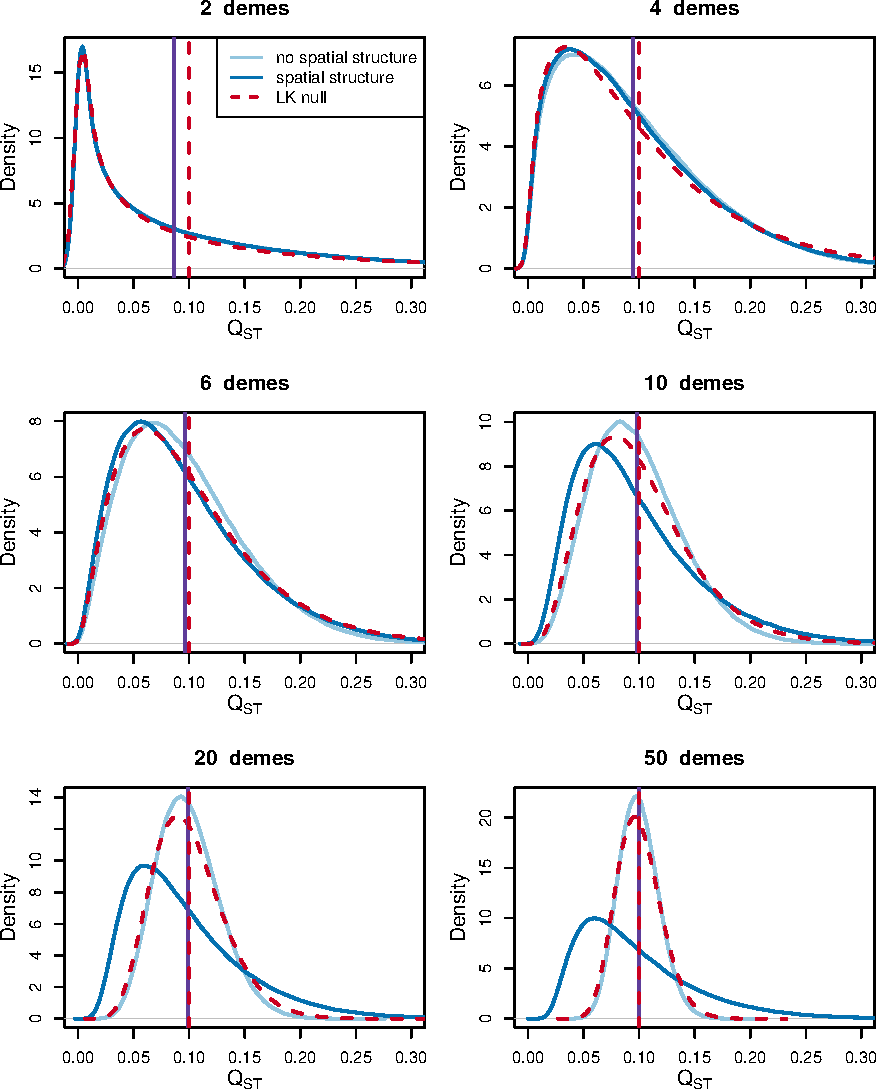
\includegraphics[width=0.8\textwidth]{qst_deme_compare.pdf}
  \caption{A comparison of the Lewontin-Krakauer (LK) distribution with the
    distribution of $Q_{ST}$ derived in this paper based on the infinitesimal
    model. A model of no spatial structure and equal migration between demes is
    compared to a stepping stone model where populations are arranged in a ring.
    $F_{ST}$ is held constant while the number of demes is increased by altering
    the migration rate.}
  \label{fig:qst_deme}
\end{figure}
\begin{figure}
  \centering
  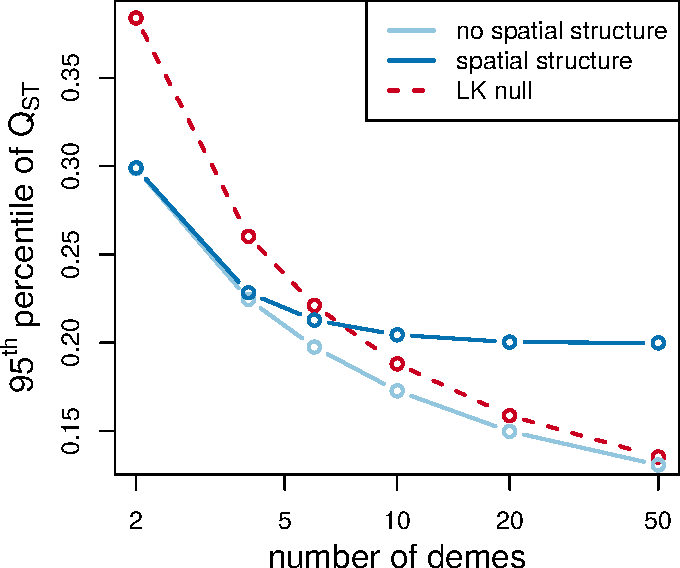
\includegraphics[width=0.5\textwidth]{qst_deme_percentile_nospace.pdf}
  \caption{Differences in the $95^{\mathrm{th}}$ percentile of the $Q_{ST}$
    distribution.}
  \label{fig:qst_perc}
\end{figure}
An obvious application of the above theory is to the neutral divergence between
groups expected in structure populations. A good place to start is by asking
what level of divergence is expected is in the infinitesimal limit. A common way
to quantify the divergence in trait value between groups is $Q_{ST}$. This is
the variance between the group means divided by the total variance in the
population. Since this study uses a haploid model, we will define
$Q_{ST} = \frac{V_{between}}{V_{between} + V_{within}}$. These variances are defined at
the population level and can be written as
\begin{equation*}
  V_{between} = \frac{1}{K} \sum_i \left( \bar{Y}_i - \bar{Y} \right)^2
\end{equation*}
and
\begin{equation*}
  V_{within} = \frac{1}{\sum_k N_k} \sum_i \sum_j \left( Y_{i,j} - \bar{Y}_i \right)^2. 
\end{equation*}

In the infinitesimal limit all $Y_{i,j}$ are normally distributed. The terms
$\bar{Y}_{i} - \bar{Y}$ and $Y_{i,j} - \bar{Y}_i$ are therefore also normal.
When population sizes are large, individual deviations from population means are
uncorrelated as are $V_{between}$ and $V_{within}$. $V_{within}$ is nearly
constant across evolutionary realizations and is equal to $\sum_k N_k
E[\tau_{kk}] / \sum_k N_k$. The between group variance is more complicated, but
its distribution can be simulated from by drawing the $\bar{Y}_{i} - \bar{Y}$ from a
multivariate normal distribution with mean zero and covariance matrix with elements
\begin{equation}
  \Cov[\bar{Y}_{i} - \bar{Y}, \bar{Y}_{j} - \bar{Y}] =
  \sigma^2(\bar{\tau}_{i,\cdot} + \bar{\tau}_{j,\cdot} - \bar{\tau}_{\cdot,\cdot} - \bar{\tau}_{i,j}).
\end{equation}
To simulate $Q_{ST}$ values it is not necessary to know $\sigma^2$. Using
expected coalescent times, perhaps measured in units of mutations, are
sufficient for simulation.

A classical result in evolutionary quantitative genetics is that $Q_{ST}=F_{ST}$
\citep{Whitlock1999}. $F_{ST}$ in this context refers to a parameter of the
population. In particular, $F_{ST} = \frac{\bar{t} - \bar{t}_0}{\bar{t}}$, where
$\bar{t}$ is the expected coalescent time for two loci sampled at random from
the entire population and $\bar{t}_0$ is the expected coalescent time for two
loci sampled within a subpopulation. This value is constant over realizations of
the evolutionary process. $Q_{ST}$ for a particular trait could refer to a state
of the population or to an estimate of this state. As shown above, $Q_{ST}$ as a
state of the population varies across evolutionary realizations. The expectation
of $V_{between}$ is $\bar{t} - \bar{t}_0$, and the expectation of $V_{within}$
is $\bar{t}_0$. $\frac{\E[V_{between}]}{\E[V_{between}] + \E[V_{within}]}$ is
equal to $F_{ST}$, but due to Jensen's inequality, $\E[Q_{ST}]$ is less
than $F_{ST}$.

The null distribution of $Q_{ST}$ derived here could be useful in
goodness-of-fit tests for whether an observed value would be unlikley under
neutrality. Current methods to perform such tests either compare $Q_{ST}$ to an
empirical distribution of $F_{ST}$ values or to a $\chi^2$ distribution. In the
second case an identical distribution to that developed by \citet{Lewontin1973}
is used. This procedure was suggested by \citet{Whitlock2009} and is implemented
in the program \textit{QstFstComp} \citep{Gilbert2015}. The Lewontin-Krakauer
(LK) distribution assumes independence between demes and provides a good
approximation in populations without spatial structure and when the number of
demes is large (Figure \ref{fig:qst_deme}). When demes are strongly correlated,
such as in spatial structured population, the LK distribution is a very poor
approximation. Even when the distributions appear similarly shaped there are
substantial differences in tail probabilities (Figure \ref{fig:qst_perc}).


\section{The response to selection}
One situation in which higher order moments of the trait distribution can be
relevant is in the response of the population to selection. The classical theory
of quantitative genetics assumes that the distribution of additive genetic
values in the population remains normally distributed as selection alters the
mean and variance. \citet{Turelli1990} used a multilocus population genetic
model to show how departures from normality can influence the response to
selection. In their analysis these departures are due to the build up of linkage
disequilibrium. However, their results are valid regardless of how the
departures from normality arise.

According to \citet{Turelli1990}, the response of the mean phenotype in the
population is 
\begin{equation}
  \label{eq:selresp}
  \Delta \bar{Z} = V_gL_1 + M_{3,g}L_2 + \gamma_4V^2_gL_3 +
  \left( M_{5,g}-4M_{3,g}V_g\right)L_4 + \ldots.
\end{equation}
Here, $Z$ refers to a phenotypic value which has an environmental component as
opposed to the trait value $Y$ which is due entirely to genetics. $V_g$ is the
variance in breeding values in the population and $\gamma_4$ is the excess
kurtosis above a normal distribution. The terms $M_{i,g}$ are the $i^{th}$
central moments of the breeding value distribution in the population. The terms
$L_i$ describe the effect of selection on the trait values and are selection
gradients in terms of the genotypic moments. In the absence of environmental
effects, or if selection acts directly on the genetic trait values, this
equation holds for the response of the mean trait value.

Equation \eqref{eq:selresp} shows that the importance of higher order moments of
the trait distribution depends on the precise shape of the fitness function. In
particular, the excess kurtosis affects the response to selection linearly with
$L_3$, the partial derivative of the log of the mean fitness with respect to the
third moment of the trait value distribution. As a very simple example we can
consider selection acting only directly on the trait values with a cubic
selection function. This can be represented by
\begin{equation}
  \label{eq:cubsel}
  W_g(Y) = b_0 + b_3(Y-\bar{Y})^3.
\end{equation}
This fitness function models selection on differences from the current mean
breeding value in the population. One thing we need to consider about the cubic
selection function is that it can give negative values for fitness, which is
obviously bad. We therefore must assume that the degree of cubic selection,
$b_3$ is not too large relative to fitness value at the population mean, $b_0$.
It turns out that the response to selection is this simply
\begin{equation}
  \label{eq:cubresp}
  \Delta \bar{Z} = \frac{M_{4,g}\beta}{1 + M_{3,g}\beta},
\end{equation}
where $\beta=b_3/b_0$. Simulations show that this predicts the response to
selection up until about $\beta\approx 2e-3$. Equation \eqref{eq:cubresp}
predicts that, holding the variance constant, the response to selection of the
mean trait value increases linearly with the kurtosis.

This is not the most realistic fitness function because it has been centered on
the mean trait value in the population. The mean will have diverged since the
most recent common ancestor of the population in the absence of stabilizing
selection making this value not so meaningful biologically. Additionally, for
the selection to be strictly cubic in shape is unrealistic. However, a large set
of fitness functions will have a component which is cubic on the trait values.
Based on this result we would expect the importance of that cubic part to depend
on the population trait kurtosis.
\section{Discussion}
The main result of this work has been to show that the characteristic function
for the distribution of trait values derived by \citet{Schraiber2015} is a
special case of the general relationship given in equation \eqref{eq:sub}. What
this implies is that to get mgf of the trait value distribution one must first
be able to write the mgf for the genealogical distribution. These functions have
been studied by \citet{Lohse2011} and in subsequent papers. They are recursive
in nature and the number of terms becomes quickly intractable as the number of
individuals increases. Things are simplified substantially when either a low
mutation approximation or infinitesimal model is used. In these cases only the
mean branch lengths or expected pair coalescent times, respectively, are
necessary to describe the trait value distribution.

The focus on kurtosis here is perhaps undue. It is presented mostly as an
example of how a simple and intuitive result can be obtained from the given
mgfs. For many traits the infinitesimal model surely provides a good null
distribution. For traits that do have sparse genetic architectures and
mutational distributions with large tails it is possible that aspects of the
mutational distribution could be learned from population samples, but it would
likely be necessary to somehow pool information across a large number of traits.
A possible instance where this could be achieved is for gene expression levels
\citep{Wheeler2016}.

It would be interesting to extend these results, which are only for the haploid,
unlinked, additive case to include factors like dominance, epistasis and
linkage. For epistasis this is likely to be very difficult since there are no
nice relationships for the mgf of a nonlinear combination of random variables.
Still, some approximations may be possible for particular forms of epistasis.
These would be of particular interest when testing for departures from
neutrality in structured populations as in \citet{Ovaskainen2011}.

\bibliographystyle{genetics} 
\bibliography{quant_gen}
\clearpage

%% APPENDIX %%
\appendix
\section{Central limit theorem for the infinitesimal model}
\label{clt}
Recall that the moment generating function for the distribution of trait values
from a single locus is
\begin{equation*}
  \varphi_{\mathbf{Y}}(\mathbf{k}) = \int \exp \left( \sum_{\omega \in \Omega} s_{\omega}t_{\omega} \right)
  \Pro(\mathbf{T}=\mathbf{t})\mathrm{d}\mathbf{t}
  \Bigr|_{s_{\omega}=\frac{\theta}{2} \left( \psi\left(\sum_{a \in \omega}k_{a}\right) -1 \right)}.
\end{equation*}
If we substitute in the Taylor series expansions for the moment generating
function of the trait value distribution we get
\begin{equation*}
  \int \prod_{\Omega} \exp\left[ t_{\omega} \T \left( \sum_{n=1}^{\infty} \frac{m_n}{n!}
    \left( \sum_{a \in \omega} k_a \right)^n \right) \right]
  \Pro(\mathbf{T} = \mathbf{t}) \mathrm{d}\mathbf{t}.
\end{equation*}
If we then write the Taylor series of each exponential function we get
\begin{equation*}
  \int \prod_{\Omega} \left[ \sum_{j=0}^\infty \frac{t_{\omega}^j}{j!}
  \left( \T \right)^j \left( \sum_{n=1}^{\infty} \frac{m_n}{n!}
  \left( \sum_{a \in \omega} k_a \right)^n \right)^j \right]
  \Pro(\mathbf{T} = \mathbf{t}) \mathrm{d}\mathbf{t},
\end{equation*}
which is equivalent to
\begin{equation*}
  1 + \sum_{\Omega} \E[T_\omega] \T \sum_{n=1}^{\infty} \frac{m_n}{n!} \left(
  \sum_{a \in \omega} k_a \right)^n +
  \sum_{\Omega \times \Omega} \frac{1}{2} E[T_{\omega_1}T_{\omega_2}]
  \sum_{n=1}^{\infty} \frac{m_n}{n!} \left(\sum_{a \in \omega_1} k_a \right)^n
  \sum_{n=1}^{\infty} \frac{m_n}{n!} \left(\sum_{a \in \omega_2} k_a \right)^n + \ldots
\end{equation*}

This is raised to the power $L$ for a trait controlled by $L$ loci. We want the
limit as the number of loci is increases while the mean and variance of the
effects of individual mutations decreases. This is expressed by the limits
$L \T m_1 \to \mu$, $L \T m_2\to \sigma^2$ and $L \T m_i\to 0$ for $i>2$ as $L \to \infty$.
The result of taking these limits is 
\begin{equation}
  \label{eq:clt}
  \exp \left( \sum_{\omega \in \Omega}\E[T_{\omega}] \left( \mu \left(
  \sum_{a \in \omega} k_a\right) + \frac{\sigma^2}{2}\left( \sum_{a \in \omega}
  k_a\right)^2\right)\right).
\end{equation}
This is multivariate normal with mean equal to $\E[T_{MRCA}]\mu$ because and
covariance equal to $\E[T_{\Omega_{a+b}}]\sigma^2$ because in the mgf for a
multivariate normal distribution the coefficient in the exponential of $k_a$ is
the mean of $Y_a$ and the coefficient of $k_ak_b$ is $2\Cov[Y_a,Y_b]$ if
$a\neq b$ and $\Var[Y_a]$ if $a=b$.

The terms with second order moments of the branch length distribution disappear
because these are $O(Lm_1)$ and $O(Lm_2)$. 
\section{Automatic moment derivations}
\label{symmath}
\section{Kurtosis derivations}
\label{kurt}
We can use the low mutation rate approximation to the moment generating function
to calculate moments of the distribution of trait vales. We'll start by
calculating the first and second moments. We start, as we did in deriving the
normal distribution, by substituting the Taylor series of the mutational mgf.
\begin{equation}
  \label{eq:mgf_approx_sub}
  \varphi_{\mathbf{Y}}(\mathbf{k}) \approx \left[ 1 + \sum_{\omega \in \Omega}
    \E[T_\omega] \T \left( m_1 \sum_{a \in \omega} k_a +
    \frac{m_2}{2!}\left( \sum_{a \in \omega} k_a\right)^2 +
    \frac{m_3}{3!}\left( \sum_{a \in \omega} k_a\right)^3 +
    \frac{m_4}{4!}\left( \sum_{a \in \omega} k_a\right)^4 \ldots \right) \right]^L
\end{equation}
We can expand this out using multinomial coefficients to get
\begin{align}
  \label{eq:mgf_approx_expand}
  \varphi_{\mathbf{Y}}(\mathbf{k}) &\approx 1 +
  L\T \sum_{\omega \in \mathcal{O}} \E[T_{\omega}]\left( m_1 \sum_{a \in \omega} k_a +
  \frac{m_2}{2}\left( \sum_{a \in \omega} k_a\right)^2 + \ldots \right) \nonumber \\
  &+ \frac{L(L-1)}{2} \left(\T\right)^2 \sum_{\omega \in \Omega} E[T_{\omega}]^2
  \left( m_1 \sum_{a \in \omega} k_a +
  \frac{m_2}{2}\left( \sum_{a \in \omega} k_a\right)^2 + \ldots \right)^2 \nonumber \\
  &+ L(L-1)\left(\T\right)^2\sum_{\omega_1, \omega_2 \in \Omega}\E[T_{\omega_1}]\E[T_{\omega_2}]
  \left( m_1 \sum_{a \in \omega_1} k_a + \ldots \right)
  \left( m_1 \sum_{a \in \omega_2} k_a + \ldots \right) + \ldots.
\end{align}
The first coefficient is $\binom{L}{L-1,1,\mathbf{0}}$, the second is
$\binom{L}{L-2,2,\mathbf{0}}$, and the third is $\binom{L}{L-2,1,1,\mathbf{0}}$.
To calculate the moments of this distribution one takes the partial derivatives
of the mgf and sets the dummy variables to zero.
\begin{equation}
  \label{eq:deriv}
  \E[Y_1^{r_1}\ldots Y_n^{r_n}] = \frac{\partial^{r_1 + \ldots + r_n}}{\partial k_1^{r_1} \ldots \partial k_n^{r_n}}
  \varphi_{\mathbf{Y}}(\mathbf{k})\Bigr|_{\mathbf{k}=0}
\end{equation}
Using this to calculate the first moment of the trait distribution we get
\begin{equation}
  \label{eq:mom1}
  \E[Y_a] \approx L\T m_1 \sum_{\omega \in \Omega_a} \E[T_\omega].
\end{equation}
The second moment is more complicated because there are $k_a^2$ terms in all
three lines of equation \ref{eq:mgf_approx_expand}.
\begin{align}
  \E[Y_a^2] &\approx L\T m_2 \sum_{\omega \in \Omega_a} E[t_\omega] \nonumber \\
  &+ \frac{L(L-1)}{2} \left(\T \right)^2 m_1^2 \sum_{\omega \in \Omega_a} 2 \E[T_\omega]^2 \nonumber \\
  &+ L(L-1) \left(\T \right)^2 m_1^2 \sum_{\omega_1 , \omega_2 \in \Omega_{a+b}} 2 \E[T_{\omega_1}]E[T_{\omega_2}]
\end{align}
Terms with $(\T)^2$ are kept because they also include a second order term of
$L$ in front of them. We can now calculated the variance using $\Var[Y]=\E[Y^2] -
\E[Y]^2$. The squared first moment can be written as
\begin{align}
  \left(L\T m_1 \sum_{\omega \in \Omega_a} \E[t_\omega] \right)^2 &=
  L^2\left(\T\right)^2 m_1^2 \sum_{\omega \in \Omega_a} \E[T_\omega]^2 \nonumber \\
  &+ L^2\left(\T\right)^2 m_1^2 \sum_{\omega_1 , \omega_2 \in \Omega_{a+b}} \E[T_{\omega_1}]\E[T_{\omega_2}].
\end{align}
Subtracting this from the second moment gives
\begin{align}
  \label{eq:var}
  \Var[Y_a] &\approx L\T m_2 \sum_{\omega \in \Omega_a} \E[T_\omega] \nonumber \\
  &- L \left(\T\right)^2 m_1^2 \sum_{\omega \in \Omega_a}\E[T_\omega]^2 \nonumber \\
  &-  2L \left(\T\right)^2 m_1^2 \sum_{\omega_1 , \omega_2 \in \Omega_{a+b}} \E[T_{\omega_1}]\E[T_{\omega_2}] \nonumber \\
  &= L\T m_2 \sum_{\omega \in \Omega_a} \E[T_\omega] -
  L\left( \T m_1 \sum_{\omega \in \Omega_a} \E[T_\omega] \right)^2 \nonumber \\
  &= L\T m_2 \E[T_{MRCA}] - L\left( \T m_1 \E[T_{MRCA}] \right)^2  \\
  &\approx L\T m_2 \E[T_{MRCA}].  \nonumber
\end{align}

Due to the large number of terms I only derive the fourth moment
of the trait
value distribution for the case when the mean mutational effect is zero. Having
the mean equal to zero is also helpful when comparing against a normal
distribution because higher order moments of the normal distribution are easy to
calculate when the mean is zero. The terms of \eqref{eq:mgf_approx_sub} that
will appear in the fourth moment after we apply \eqref{eq:deriv} are
\begin{equation*}
  L \left(\T\right) \frac{m_4}{24}
  \sum_{\omega \in \Omega_a} \E[T_\omega] \left(\sum_{a \in \omega} k_a\right)^4
\end{equation*}
for the fourth moment along one branch,
\begin{equation*}
  \binom{L}{L-2,2,\mathbf{0}}\left(\T\right)^2\left(\frac{m_2}{2}\right)^2
  24 \sum_{\omega \in \Omega_a} \E[T_\omega]^2 \left(\sum_{a \in \omega} k_a\right)^4
\end{equation*}
for the second moment of the same branch chosen twice, and
\begin{equation*}
  \binom{L}{L-2,1,1,\mathbf{0}}\left(\T\right)^2\left(\frac{m_2}{2}\right)^2
  24 \sum_{\omega_1 , \omega_2 \in \Omega_{a+b}} \E[T_{\omega_1}]\E[T_{\omega_2}]
  \left(\sum_{a \in \omega_1} k_a\right)^2\left(\sum_{a \in \omega_2} k_a\right)^2
\end{equation*}
for the second moments on two different branches. Taking the fourth derivatives
of these in terms of the desired branch we get
\begin{align}
  \label{eq:mom4}
  \E[Y_a^4] &= L\T m_4 \E[T_{MRCA}] \nonumber \\
  &+ \frac{L(L-1)}{2} \left(\T\right)^2\left( \frac{m_2}{2} \right)^2
  24 \sum_{\omega \in \Omega_a} \E[t_\omega]^2 \nonumber \\
  &+ L(L-1) \left(\T\right)^2\left( \frac{m_2}{2} \right)^2
  24 \sum_{\omega_1 , \omega_2 \in \Omega_{a+b}} \E[T_{\omega_1}]\E[T_{\omega_2}] \nonumber \\
  &= L\T m_4 \E[T_{MRCA}] +
  3L(L-1)\left( \T m_2 \sum_{\omega \in \Omega_a} \E[T_\omega] \right)^2x \nonumber \\
  &= L\T m_4 \E[T_{MRCA}] +
  3L(L-1)\left( \T m_2 \E[T_{MRCA}] \right)^2 \\
  &\approx L\T m_4 \E[T_{MRCA}] +
  3\left(L \T m_2 \E[T_{MRCA}] \right)^2. \nonumber 
\end{align}

The kurtosis is defined as
\begin{equation*}
  Kurt[X]=\frac{E[(X-E[X])^4]}{E[(X-E[X])]^2]^2.}
\end{equation*}
This is the fourth central moment divided by the variance. For ease of
calculation, we'll examine this in the case where the mean mutation effect (and
therefore trait value) is zero. If we plug \eqref{eq:var} and \eqref{eq:mom4}
into the expression for the kurtosis we get
\begin{align*}
  \Kurt[Y_a] &= \frac{L\T m_4 \E[T_{MRCA}]}{\left(L\T m_2 \E[T_{MRCA}]\right)^2} +
  \frac{3L(L-1)\left( \T m_2  \E[T_{MRCA}]\right)^2}{\left(L\T m_2 \E[T_{MRCA}]\right)^2} \nonumber \\
  &= \frac{m_4}{L\T m_2^2\E[T_{MRCA}]} + \frac{3(L^2-L)}{L^2} \nonumber \\
  &= \frac{\kappa}{L\T \E[T_{MRCA}]} + 3\left( 1 - \frac{1}{L} \right).
\end{align*}

We also calculate here some additional moments that have less clear
interpretations but are useful later on when calculating the expected population
kurtosis. The first of these is $\E[Y_a^3Y_b]$. The terms of
\eqref{eq:mgf_approx_sub} that will appear in this are
\begin{equation*}
  L \left(\T\right) \frac{m_4}{24} 4 k_a^3k_b \sum_{\omega \in \Omega_{a+b}} \E[T_\omega]
\end{equation*}
and
\begin{equation*}
  L(L-1)\left(\T \frac{m_2}{2}\right)^2 k_a^2 \times 2k_ak_b
  \left( \sum_{\omega \in \Omega_{a+b}} \E[T_\omega] \right) \left( \sum_{\omega \in \Omega_a} \E[T_\omega] \right).
\end{equation*}
This ultimately gives
\begin{equation}
  \label{eq:m31}
  E[Y_a^3Y_b] = L \T m_4 \E[\tau_{a+b}] + 3L(L-1) \left(\T m_2\right)^2 \E[T_{MRCA}]\E[\tau_{a+b}].
\end{equation}
The next fourth moment of interest is $\E[Y_a^2Y_bY_c]$. The terms of
\eqref{eq:mgf_approx_sub} are
\begin{equation*}
  L \T \frac{m_4}{24} 12k_a^2k_bk_c \sum_{\omega \in \Omega_{a+b+c}} \E[T_\omega],
\end{equation*}
\begin{equation*}
  L(L-1) \left(\T \frac{m_2}{2}\right)^2 k_a^2 \times 2k_bk_c
  \left( \sum_{\omega \in \Omega_a} \E[T_\omega] \right)\left( \sum_{\omega \in \Omega_{a+b}} \E[T_\omega] \right),
\end{equation*}
and 
\begin{equation*}
  L(L-1) \left(\T \frac{m_2}{2}\right)^2 2k_ak_b \times 2k_ak_c \left( \sum_{\omega \in \Omega_{a+b}} \E[T_\omega] \right)
  \left( \sum_{\omega \in \omega_{b+c}} \E[T_\omega] \right).
\end{equation*}
Taking the appropriate derivatives of these gives
\begin{equation}
  \label{eq:m211}
  L \T m_4 \E[\tau_{a+b+c}] + L(L-1)\left(\T m_2\right)^2\E[T_{MRCA}]\E[\tau_{b+c}] +
  2L(L-1) \left(\T m_2\right)^2\E[\tau_{a+b}]\E[\tau_{a+c}].
\end{equation}
Individuals in the population are exchangeable as long as it is not structured.
The pairwise expected shared branch lengths are in that case all equal and we
can write \eqref{eq:m211} as
\begin{equation}
  \label{eq:m211s}
  L \T m_4 \E[\tau_{a+b+c}] + L(L-1)\left(\T m_2\right)^2\E[T_{MRCA}]\E[\tau_{a+b}] +
  2L(L-1) \left(\T m_2\right)^2\E[\tau_{a+b}]^2.
\end{equation}
Where $\tau_{a+b}$ just refers to the expected shared branch length of any two
individuals in the population. The final moment we'll look at is
$\E[Y_aY_bY_cY_d]$ which has relevant terms
%% The set of branches containing all individuals
\begin{equation*}
  L \T \frac{m_4}{24} 24k_ak_bk_ck_d \sum_{\omega \in \Omega_{a+b+c+d}} \E[T_\omega],
\end{equation*}
%% Cross set of a-b branches and c-d branches
\begin{equation*}
  L(L-1) \left(\T \frac{m_2}{2}\right)^2 2k_ak_b \times 2k_ck_d \left( \sum_{\omega \in \Omega_{a+b}} \E[T_\omega] \right)
  \left( \sum_{\omega \in \Omega_{c+d}} \E[T_\omega] \right),
\end{equation*}
%% Cross set of a-c branches and b-d branches
\begin{equation*}
  L(L-1) \left(\T \frac{m_2}{2}\right)^2 2k_ak_c \times 2k_bk_d \left( \sum_{\omega \in \Omega_{a+c}} \E[T_\omega] \right)
  \left( \sum_{\omega \in \Omega_{b+d}} \E[T_\omega] \right),
\end{equation*}
and
%% cross set of a-d branches and b-c branches
\begin{equation*}
  L(L-1) \left(\T \frac{m_2}{2}\right)^2 2k_ak_d \times 2k_bk_c \left( \sum_{\omega \in \Omega_{a+d}} \E[T_\omega] \right)
  \left( \sum_{\omega \in \omega_{b+c}} \E[T_\omega] \right).
\end{equation*}
When the appropriate fourth order partial derivatives are taken of this we get
\begin{align*}
  L \T m_4 \E[\tau_{a+b+c+d}] \\
  + L(L-1)\left(\T m_2\right)^2\E[\tau_{a+b}]\E[\tau_{c+d}] \\
  + L(L-1)\left(\T m_2\right)^2\E[\tau_{a+c}]\E[\tau_{b+d}] \\
  + L(L-1)\left(\T m_2\right)^2\E[\tau_{a+d}]\E[\tau_{b+c}].
\end{align*}
We can again simplify this expression for populations with exchangeable
individuals. This gives
\begin{equation}
  \label{eq:m1111}
  L \T m_4 \E[\tau_{a+b+c+d}] + 3L(L-1)\left(\T m_2\right)^2\E[\tau_{a+b}]^2.
\end{equation}

The expected kurtosis in the population is a quotient and therefore annoying to
calculate. Instead we will calculate the expected fourth central moment. 
\begin{equation}
  \E[M_{4,Y}] = \E\left[\frac{1}{N} \sum \left( Y_i - \frac{\sum Y_j}{N} \right)^4 \right].
\end{equation}
Examining the sum inside the expectation we see that 
\begin{align}
  \label{eq:expandkurt}
  \E\left[ \left( Y_i - \frac{\sum Y_j}{N} \right)^4 \right] &= \E[Y_i^4] - 
                                                              4\E\left[ Y_i^3 \frac{\sum Y_j}{N} \right] + 
                                                              6\E\left[Y_i^2\left(\frac{\sum Y_j}{N}\right)^2\right] - 
                                                              4\E\left[Y_i\left(\frac{\sum Y_j}{N}\right)^3\right]+ 
                                                              \left(\frac{\sum Y_j}{N}\right)^4 \nonumber \\
                                                            &= \E[Y_i^4] - 
                                                              \frac{4}{N}\sum_j \E[Y_i^3Y_j] + 
                                                              \frac{6}{N^2}\sum_{j,k} \E[Y_i^2Y_jY_k] \nonumber\\
                                                              &-\frac{4}{N^3}\sum_{j,k,l}\E[Y_iY_jY_kY_l] + 
                                                              \frac{1}{n^4}\sum_{j,k,l,d}\E[Y_jY_kY_lY_d].
\end{align}
In calculating these expectations we have to remember that the value depends
only on the number of times each variable appears in the expectation. That is,
$\E[Y_1^2Y_2Y_3]$ is equivalent to $\E[Y_1Y_2^3Y_3]$ as long as all individuals in
the population are exchangeable. The resulting expansion of
\eqref{eq:expandkurt} is therefore quite ugly. It can be simplified by only
considering terms of order one. Other terms can be ignored since we are
assuming there are a fair number of individuals in the population. This yields
\begin{align}
  \label{eq:popkurt}
  \E\left[ \left( Y_i - \frac{\sum Y_j}{N} \right)^4 \right] &=
  \E[Y_i^4]  - \frac{4(n-1)}{n}\E[Y_i^3Y_j] + \frac{6(n-1)(n-2)}{n^2}\E[Y_i^3Y_jY_k]  \nonumber \\
  &- \frac{4(n-1)(n-2)(n-3)}{n^3}\E[Y_iY_jY_kY_l] \nonumber \\
  &+ \frac{(n-1)(n-2)(n-3)(n-4)}{n^4}\E[Y_jY_kY_lY_d]
  + O(n^{-1}) \nonumber \\
  &\approx \E[Y_i^4]  - 4\E[Y_i^3Y_j] + 6\E[Y_i^2Y_jY_k] - 3\E[Y_iY_jY_kY_l].
\end{align}

The first term, $\E[Y_i^4]$ was derived in equation \eqref{eq:mom4} as
\begin{equation*}
  L\T m_4 \E[T_{MRCA}] + 3L(L-1)\left( \T m_2 \E[T_{MRCA}] \right)^2.
\end{equation*}
The second term, $\E[Y_i^3Y_j]$ was derived in equation \eqref{eq:m31} as
\begin{equation*}
  L \T m_4 \E[\tau_{a+b}] + 3L(L-1) \left(\T m_2\right)^2 \E[T_{MRCA}]\\E[\tau_{a+b}].
\end{equation*}
The third term, $\E[Y_i^2Y_jY_k]$ was derived in equation \eqref{eq:m211} as
\begin{equation*}
  L \T m_4 \E[\tau_{a+b+c}] + L(L-1)\left(\T m_2\right)^2\E[T_{MRCA}]\E[\tau_{a+b}] +
  2L(L-1) \left(\T m_2\right)^2\E[\tau_{a+b}]^2.
\end{equation*}
The fourth term, $\E[Y_iY_jY_kY_l]$ was derived in equation \eqref{eq:m1111} as
\begin{equation*}
  L \T m_4 \E[\tau_{a+b+c+d}] + 3L(L-1)\left(\T m_2\right)^2\E[\tau_{a+b}]^2.
\end{equation*}
Plugging these into \eqref{eq:popkurt} we get
\begin{align}
  \label{eq:popm4coal}
  \E[M_{4,Y}] &\approx L \T m_4 \left( \E[T_{MRCA}] - 4\E[\tau_{a+b}] + 6\E[\tau_{a+b+c}] -3\E[\tau_{a+b+c+d}] \right)\nonumber \\
  &+ 3\left( L \T m_2 \right)^2\left(\E[T_{MRCA}]- \E[\tau_{a+b}]\right)^2.
\end{align}
These expressions approximate $L(L-1)$ as $L^2$ as part of the low mutation rate
approximation. The fourth central moment of a normal distribution is
$3\sigma^4$. Using the expected population  variance we get $3\left(L\T m_2
\E[T_{MRCA}]- \E[\tau_{a+b}]\right)^2$. It is clear from \eqref{eq:popm4coal} that
as $L\T$ gets large the second term will dominate and the population will have
the same expected kurtosis as a normal distribution. The expected population kurtosis
is
\begin{equation*}
  \E[\mbox{Kurt}] \approx 3 + \frac{\kappa( \E[T_{MRCA}] - 4\E[\tau_{a+b}] +
    6\E[\tau_{a+b+c}] -3\E[\tau_{a+b+c+d}])}{L \T \E[T_{MRCA}]- \E[\tau_{a+b}]}.
\end{equation*}
This expression can be written in an easier to interpret form by noting that
$\E[\tau_{a+b}]=\E[T_{MRCA}] - \E[T_2]$, $\E[\tau_{a+b+c}]=\E[T_{MRCA}] - \E[T_3]$,
$\E[\tau_{a+b+c+d}]=\E[T_{MRCA}] - \E[T_4]$, where $T_i$ is the expected time it
takes for $i$ lineages to coalesce.
\begin{equation}
  \label{eq:popkurtcoal}
  \E[\mbox{Kurt}] \approx 3 + \frac{\kappa( 4T_2 - 6T_3 + 3T_4)}{L \T T_2}.
\end{equation}
In a constant size population this would be $3 + \frac{\kappa}{2L\T}$.
\end{document}
